\section{Methodology}
We introduce a novel framework incorporating multiple modalities for building atmospheric visibility estimation solutions, as well as constructing a dataset that includes both ground-level and elevated altitude conditions. 

\subsection{SeeSet V1 Dataset}
\label{sec:seeset}
To overcome the limitations encountered in the previous studies and to include a broader range of real-world scenarios, we collect a novel aerial imagery dataset SeeSet v1. This dataset was carefully curated to incorporate dynamic views capturing sceneries from multiple locations, encompassing ground-based and aerial perspectives. 

This section presents a detailed description of the data collection and labeling process (\cref{data_collection}). 
In \cref{modalities}, we present the extraction techniques used to generate the additional image modalities. 


\subsubsection{Dataset Collection Process}
\label{data_collection}

To generate our synthetic dataset, we utilize an FAA-approved flight simulator. This advanced simulator facilitates the controlled acquisition of images, showcasing diverse viewpoints and a range of visibility degradations. The process, as illustrated in Figure~\ref{fig:data_collection_process}, starts at ground-level altitude. We systematically increased visibility in incremental steps, extending up to 100 miles. Subsequently, when the visibility reaches the limit, we elevate the viewpoint's altitude and then reset the visibility to 0, continuing this procedure up to a maximum of 2000 feet AGL.


\begin{figure}[htbp]
\centerline{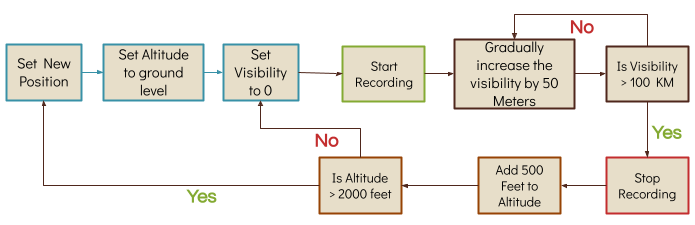
\includegraphics[width=250pt]{imgs/data_collection_pipeline.png}}
\caption{Automatic Dataset Collection Process using X-Plane 11}
\label{fig:data_collection_process}
\end{figure}
 

The collected images are automatically labeled into five discrete bins, each tailored to specific \href{https://www.faa.gov/air_traffic/publications/atpubs/aim_html/}{FAA requirements}. This categorization is based on visibility conditions and regulations relevant to both ground-based and aerial environments. The designated bins serve as the basis for the five labels utilized in training our DL models. 
We report the classes (bins) specifications and the corresponding counts in \cref{tab:vis_img_count}.


\begin{figure}
  \centering
  \begin{subfigure}[b]{0.15\textwidth}
    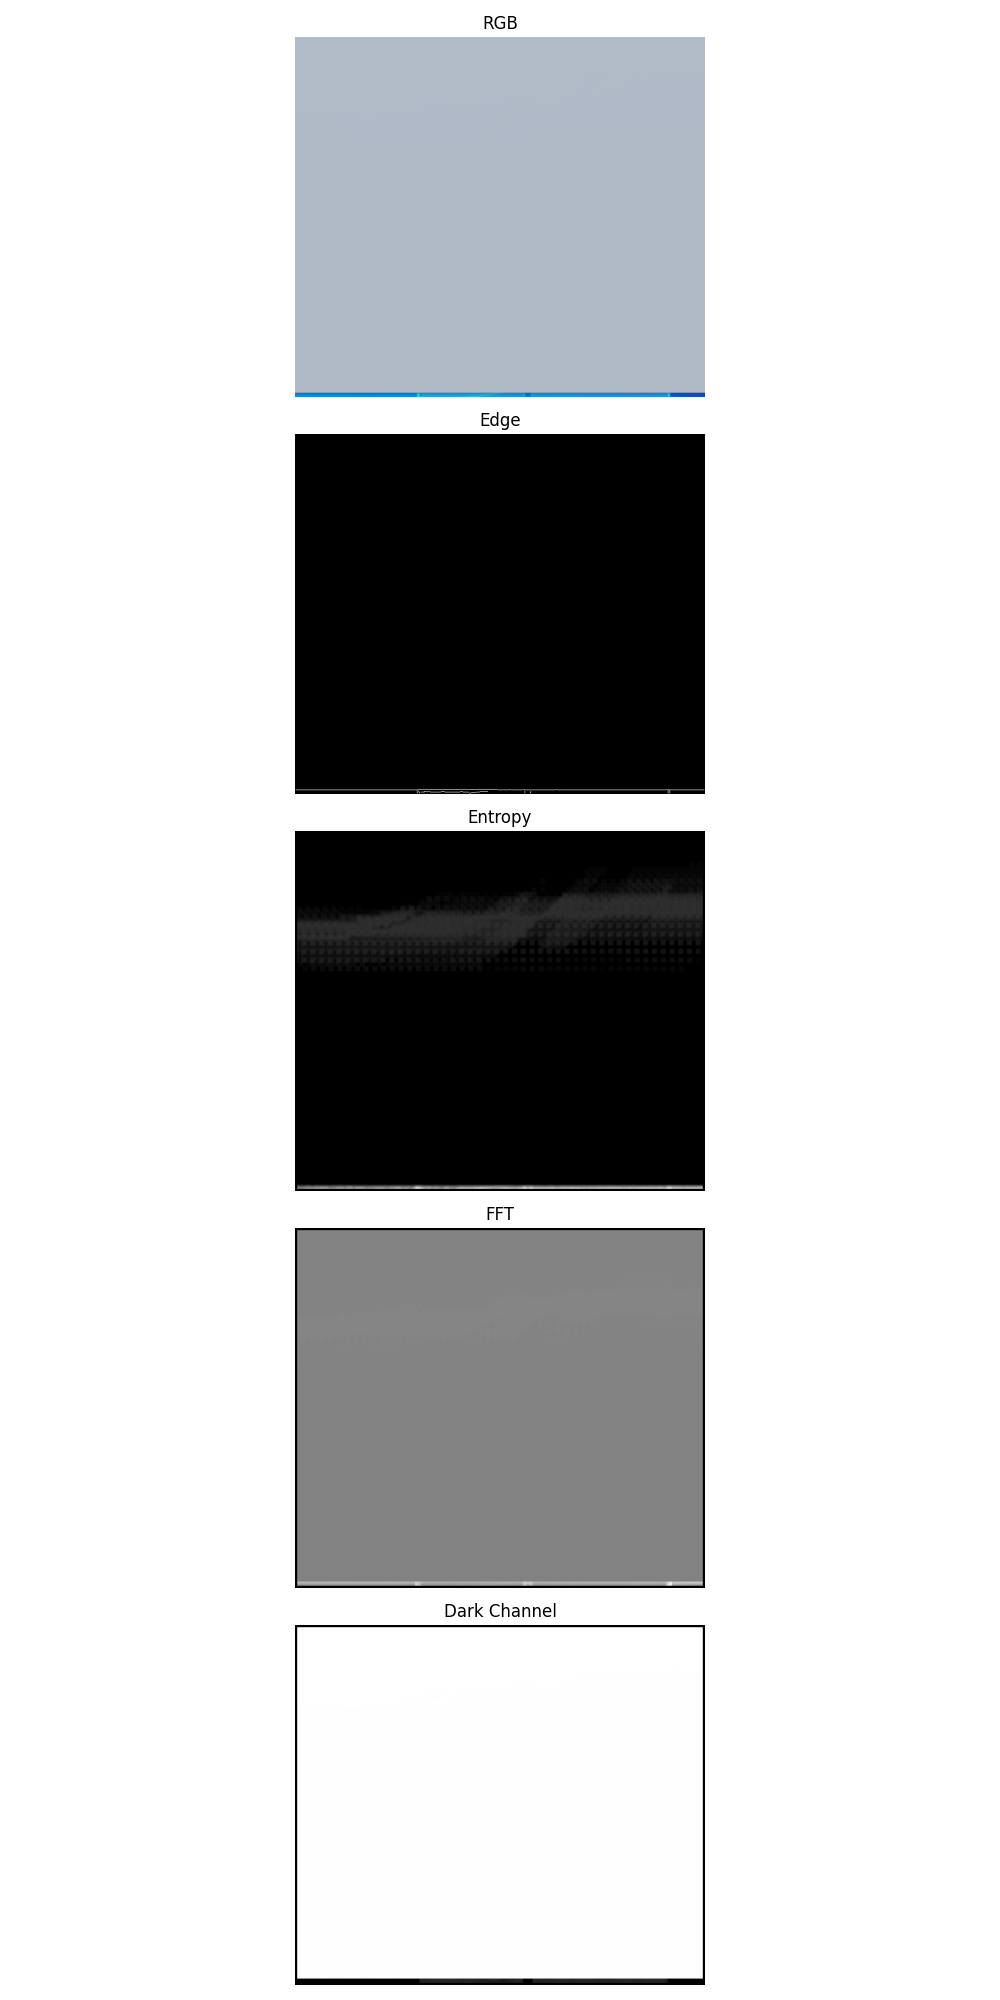
\includegraphics[width=\textwidth, trim={7.5cm 0cm 7.5cm 0cm},clip]{imgs/examples/exp_0_featuresMiles_0.12427454732996136_featuresM_200_features.png}
    \caption{< 0.5 mile}
    \label{subfig:bin0}
  \end{subfigure}
  \begin{subfigure}[b]{0.15\textwidth}
    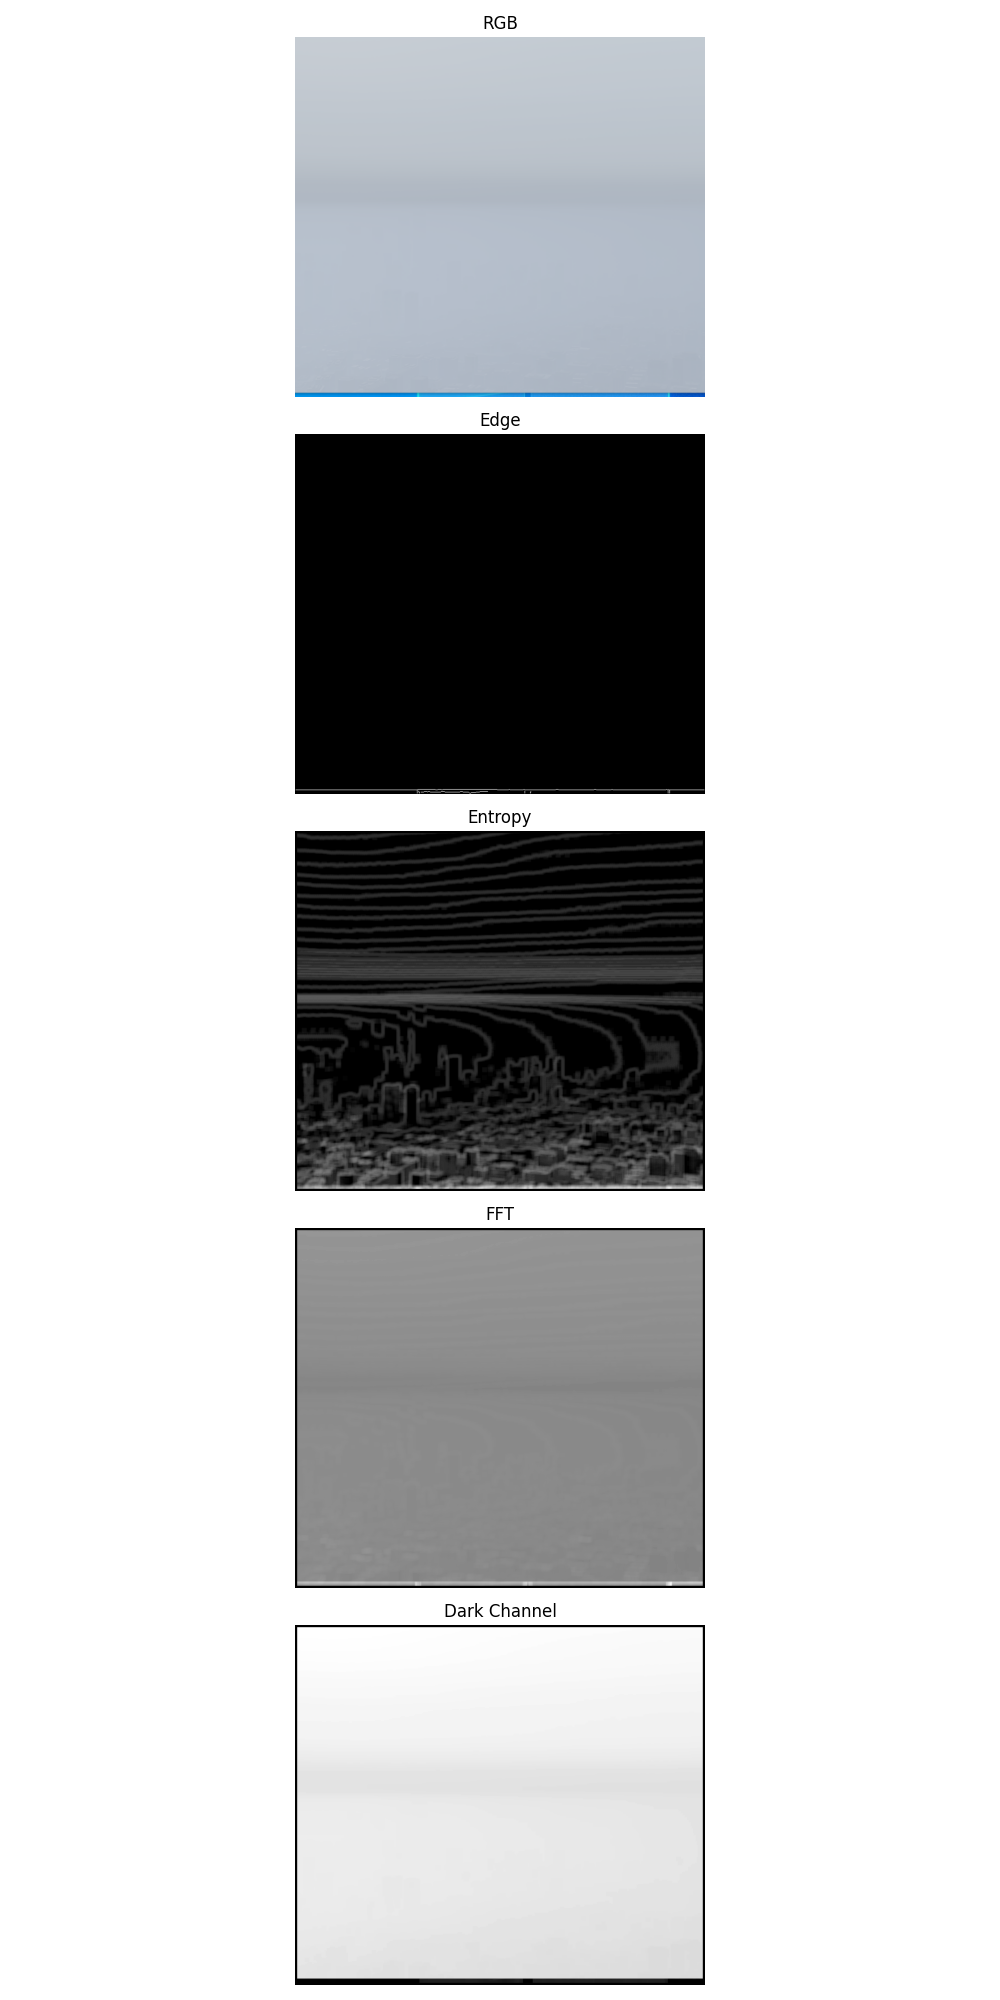
\includegraphics[width=\textwidth, trim={7.5cm 0 7.5cm 0},clip]{imgs/examples/exp_0_featuresMiles_0.9320591049747102_featuresM_1500_features.png}
    \caption{(0.5, 1] miles}
    \label{subfig:bin1}
  \end{subfigure}
  % Add the subfigrow environment here
    \begin{subfigure}[b]{0.15\textwidth}
      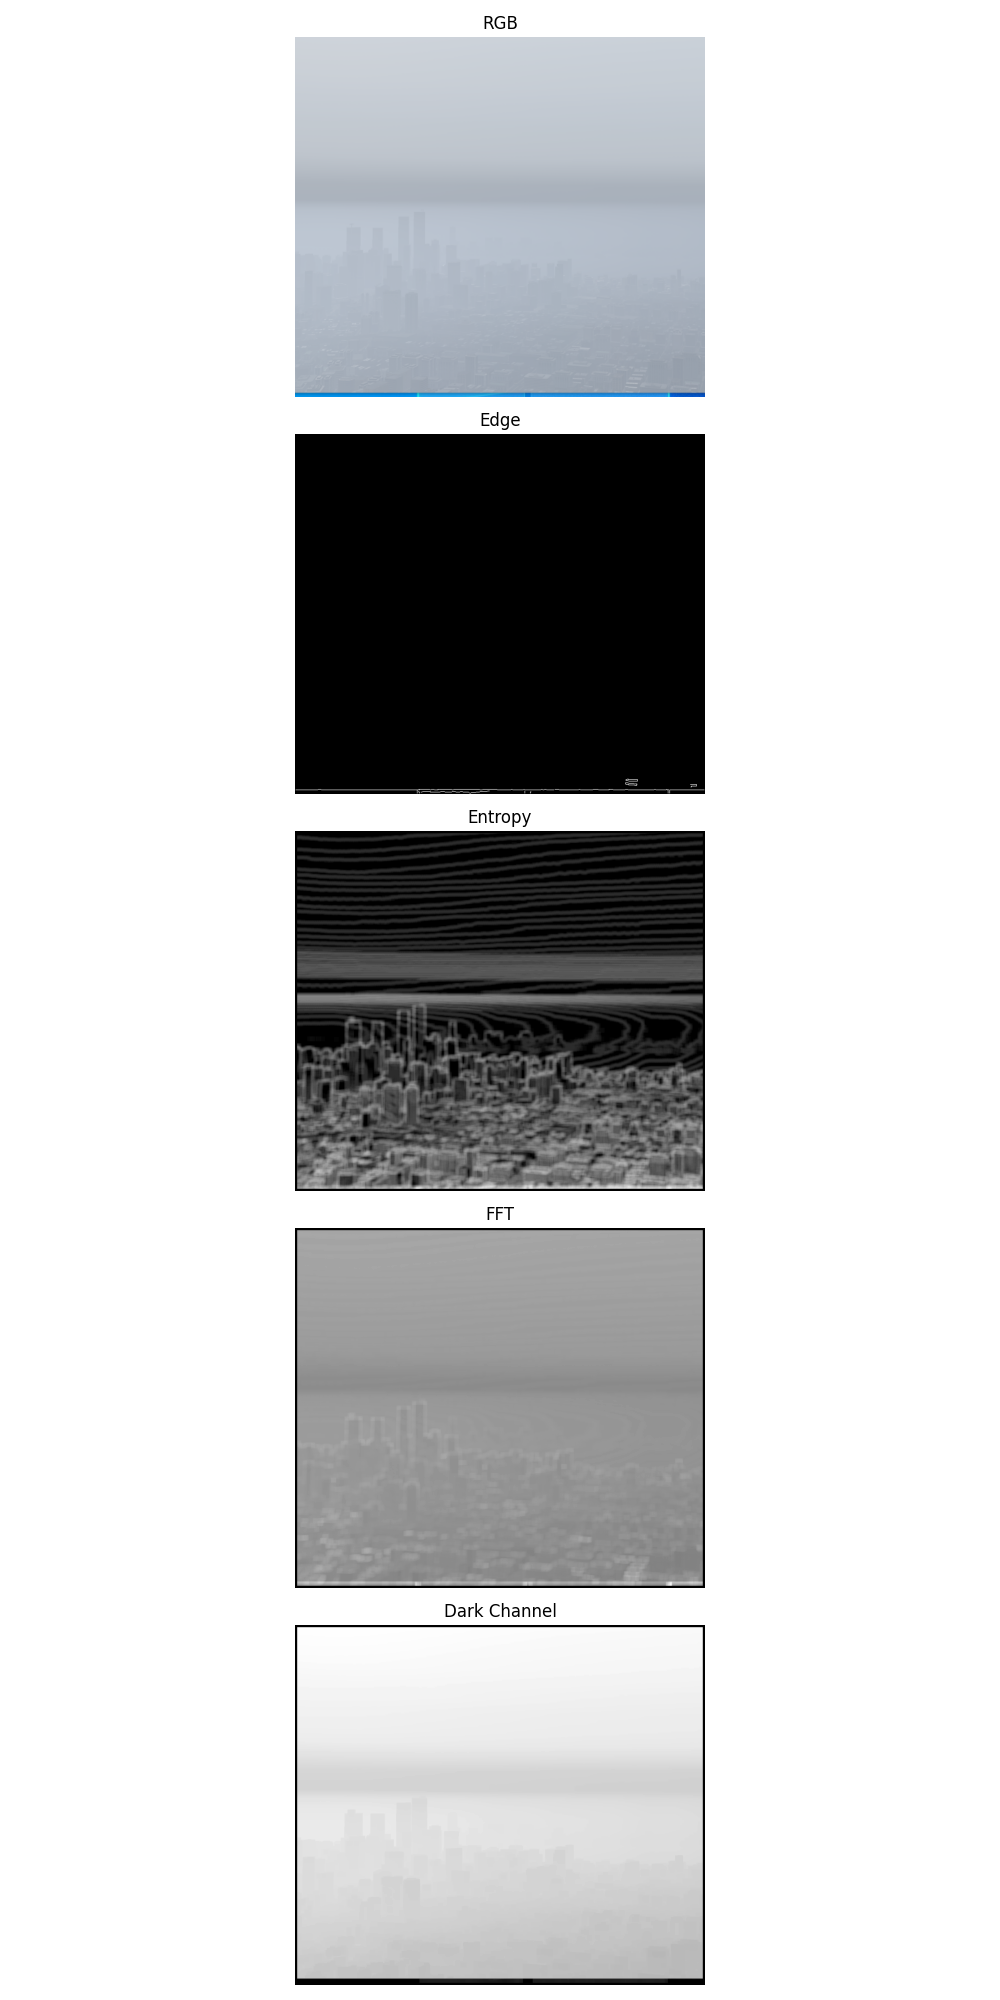
\includegraphics[width=\textwidth, trim={7.5cm 0 7.5cm 0},clip]{imgs/examples/exp_0_featuresMiles_1.8951868467819106_featuresM_3050_features.png}
      \caption{(1, 3] miles}
      \label{subfig:bin2}
    \end{subfigure}
    \begin{subfigure}[b]{0.15\textwidth}
      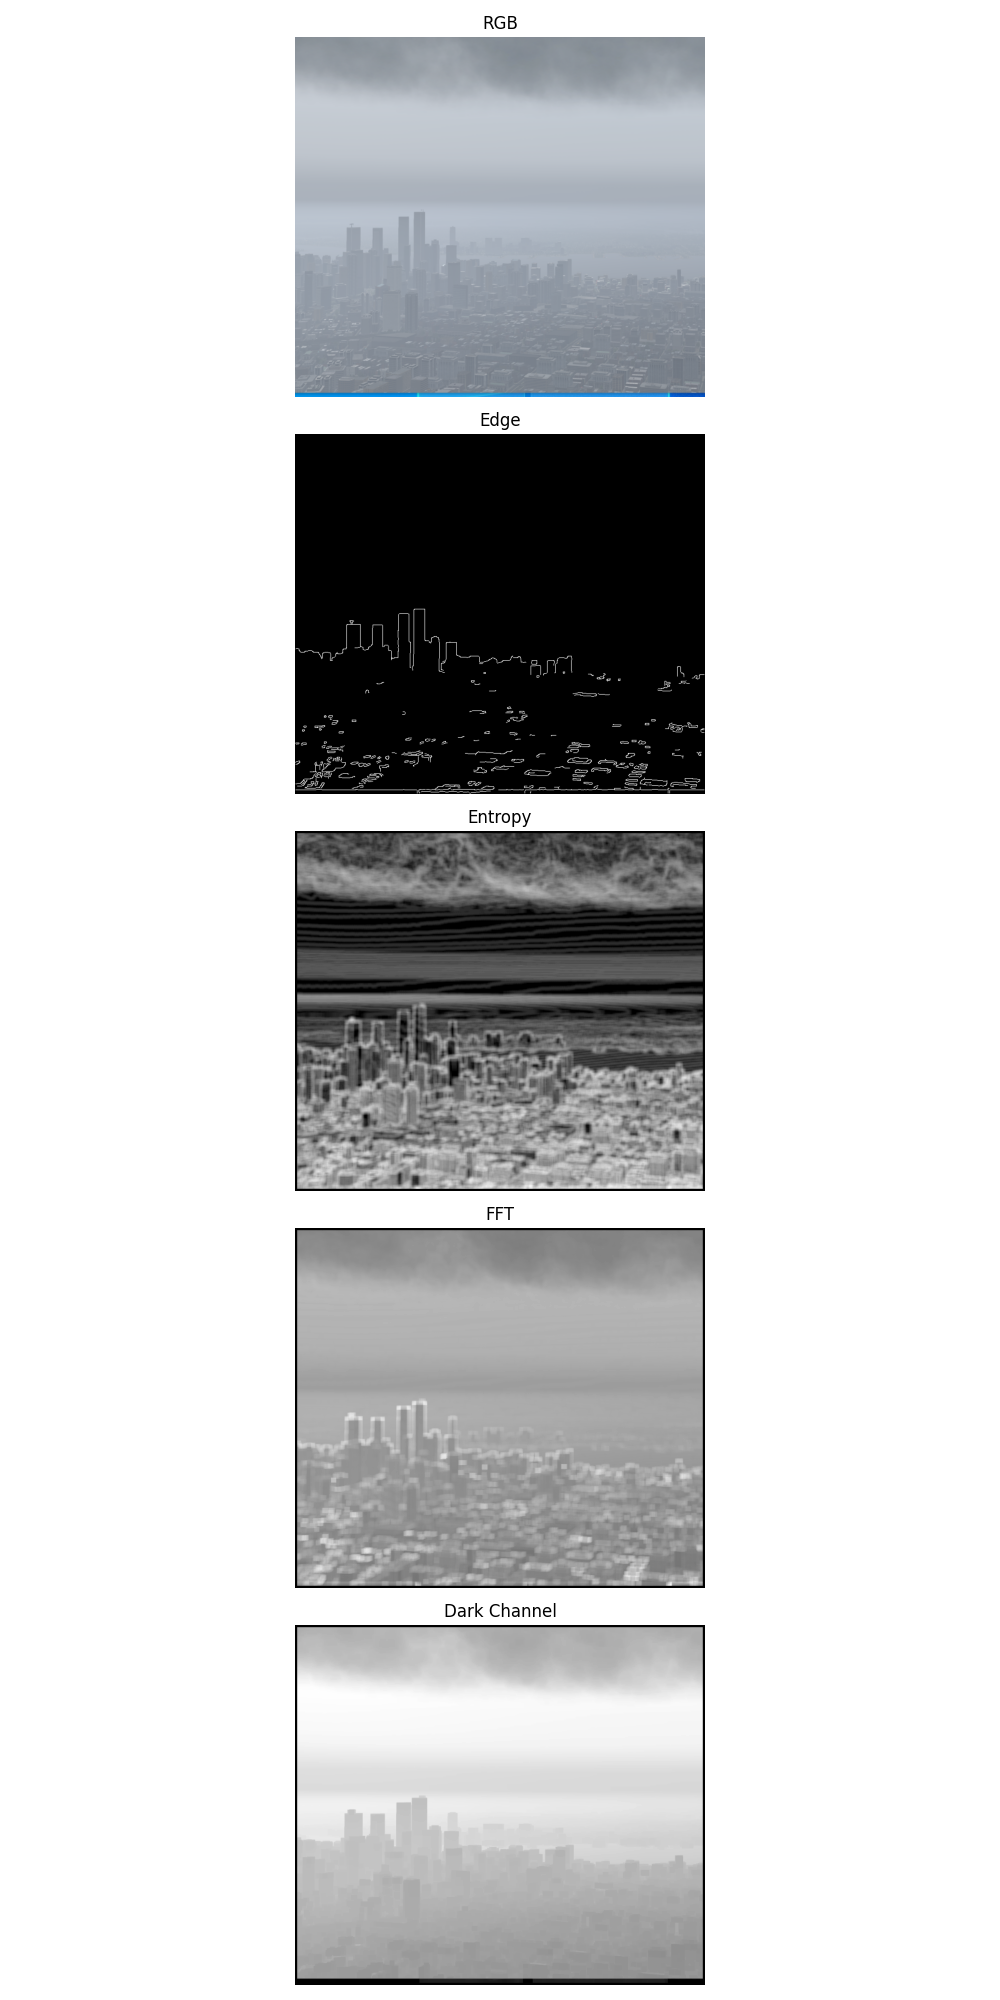
\includegraphics[width=\textwidth, trim={7.5cm 0 7.5cm 0},clip]{imgs/examples/exp_0_featuresMiles_4.038922788223744_featuresM_6500_features.png}
      \caption{(3, 5] miles}
      \label{subfig:bin3}
    \end{subfigure}
    \begin{subfigure}[b]{0.15\textwidth}
      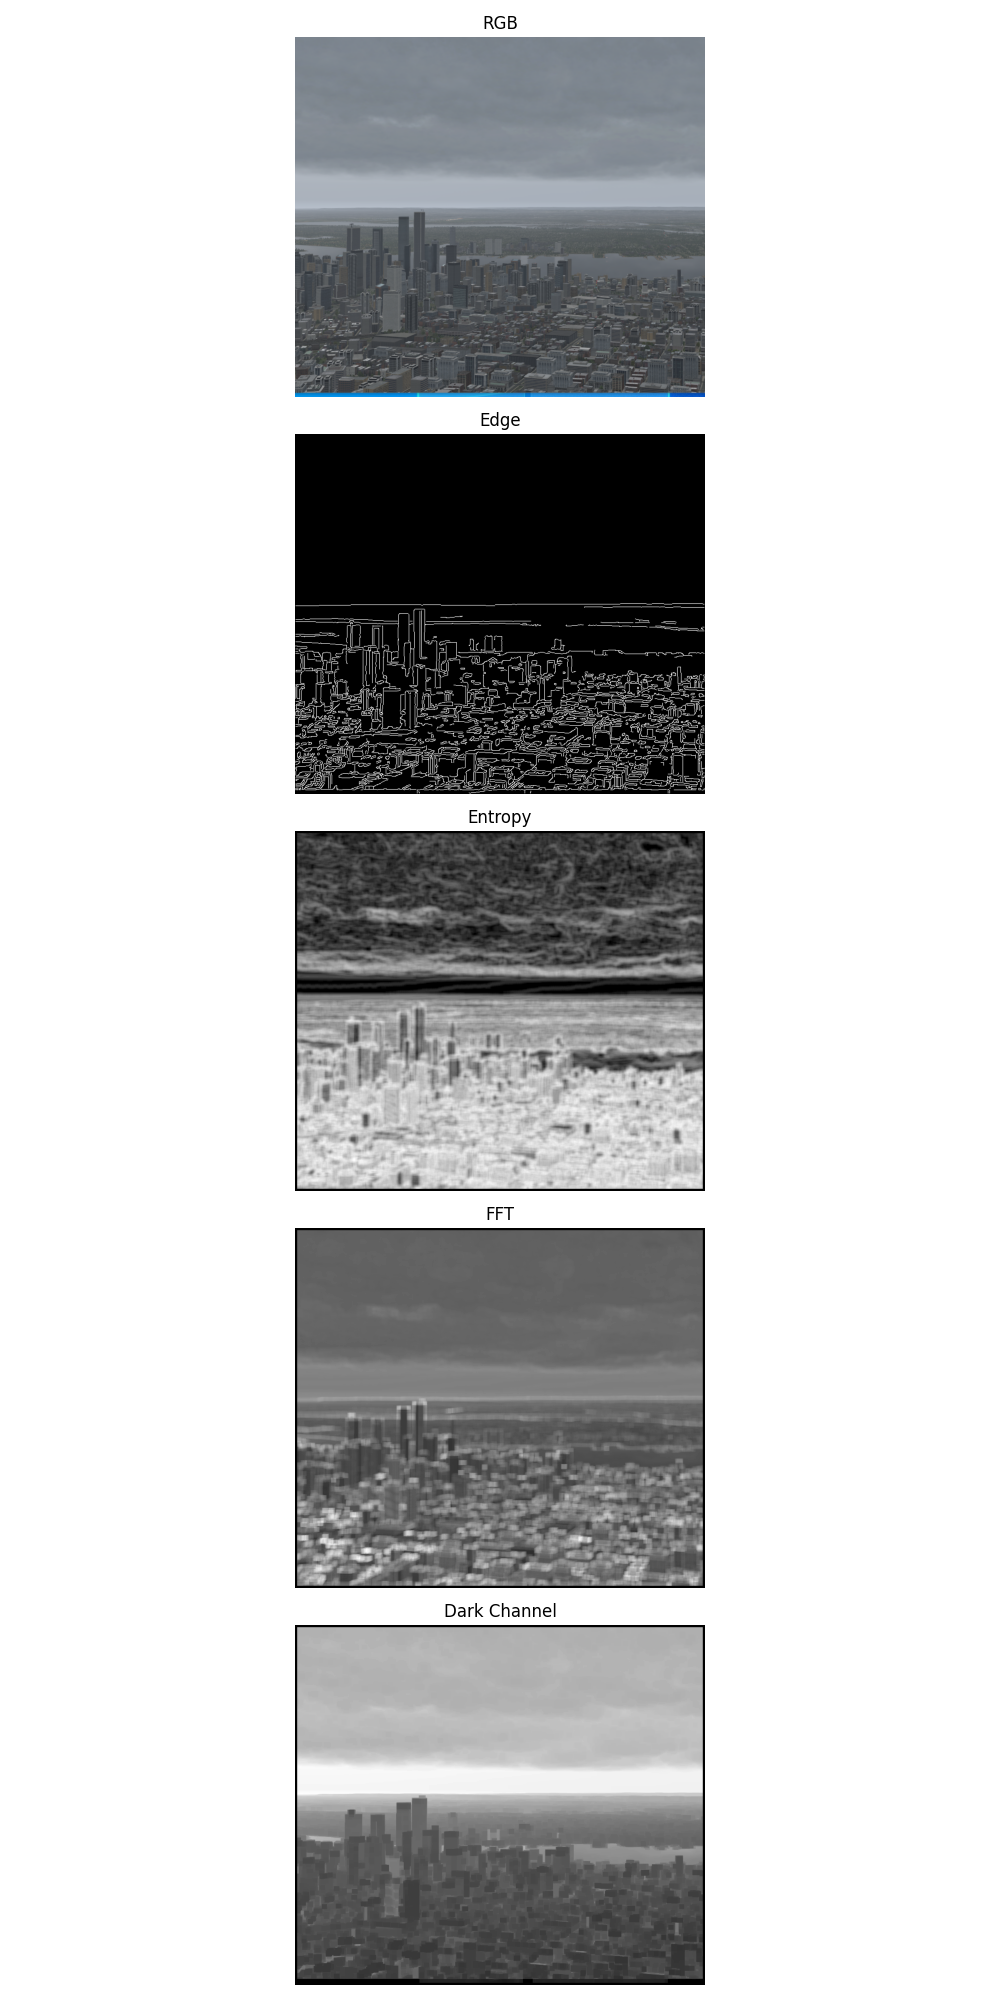
\includegraphics[width=\textwidth, trim={7.5cm 0 7.5cm 0},clip]{imgs/examples/exp_0_featuresMiles_46.1462462872979_featuresM_74265_features.png}
      \caption{> 5 miles}
      \label{subfig:bin4}
    \end{subfigure}
  
  \caption{The impact of visibility on the multiple modalities for the 6N7 Sealane 01 View. Each row shows one modality: RGB, edge map, entropy map, FFT magnitude, and dark channel prior. Each column refers to a visibility bin.}
  \label{fig:impact_vis_deg_features}
\end{figure}


\begin{table}[htbp]
\centering
\caption{Visibility Categories and Images Count}
\label{tab:vis_img_count}
\begin{tabular}{@{}lllr@{}}
\toprule
Category & Visibility in miles  & Visibility in meters & Count  \\
\midrule
4        & $\geq$ 5 miles             &     $\geq$ 8046.72m                 & 67002  \\
3        & 3 to 5 miles         &      4828.03m to  8046.72m        & 19584  \\
2        & 1 to 3 miles         &            1609.34m to 4828.03m         & 19648  \\
1        & 0.5 to 1 mile  &               804.672m to 1609.34m      & 4928  \\
0        & $\leq$ 0.5 mile   &     $\leq$ 804.672m                 & 4938  \\
\midrule
Total    &    &                      &  116100  \\
\bottomrule
\end{tabular}
\end{table}


\subsubsection{Modalities}
\label{modalities}
\textbf{Monocular Depth Estimation:}

In our approach, we used the Omnidata toolkit to extract depth maps from monocular images \cite{eftekhar2021omnidata, ranftl2021vision}. This toolkit provides a comprehensive and scalable method for depth estimation, essential for understanding the spatial arrangement in a scene. The generated depth maps offer a pixel-wise measurement of distance from the viewpoint, aiding in the accurate representation of the three-dimensional structure of the scene. 

While depth maps offer valuable information, the models employed to generate them exhibit a notable limitation when applied to our data. The training methodology involves masking the sky and exclusively considering the ground before depth estimation. This approach may pose challenges with certain images in our dataset, as they are collected at varying altitudes.

\textbf{Normal Surface Estimation:}

Alongside depth maps, we also used the Omnidata toolkit for normal surface estimation \cite{eftekhar2021omnidata}. This modality provides information about the orientation of surfaces in the image, which is crucial for understanding the geometric properties of the scene. Unlike depth estimation, this modality estimator considers both sky and ground details.


\textbf{Entropy Map:}

We incorporate an image entropy map as a modality to enhance the model's sensitivity to changes in visibility, especially in low-visibility conditions. The entropy map quantifies the amount of information present in different regions of an image. 
% We report the procedure implemented to generate the Entropy Maps in Algorithm \ref{alg:entropy_map}.


% \begin{algorithm}[htbp]
% \caption{Calculate Entropy Map}\label{alg:entropy_map}
% \begin{algorithmic}[1]
% \Require An image $I$ represented as a 2D array, window size $w$
% \Ensure Entropy map $E$ of the same dimensions as $I$
% \State $E \gets \text{zeros\_like}(I)$ \Comment{Initialize entropy map $E$ with zeros}
% \State $rows, cols \gets$ dimensions of $I$ \Comment{Get the number of rows and columns of $I$}
% \For{$i \gets 0$ \textbf{to} $rows - w$} \Comment{Iterate over rows}
%     \For{$j \gets 0$ \textbf{to} $cols - w$} \Comment{Iterate over columns}
%         \State $window \gets I[i : i+w, j : j+w]$ \Comment{Extract $w \times w$ window from $I$}
%         \State $hist \gets \text{calculateHistogram}(window)$ \Comment{Calculate histogram of the window}
%         \State $hist \gets hist / \text{sum}(hist)$ \Comment{Normalize histogram}
%         \State $entropy \gets -\sum (hist \cdot \log_2(hist + \epsilon))$ \Comment{Compute entropy}
%         \State $E[i + \frac{w}{2}, j + \frac{w}{2}] \gets entropy$ \Comment{Assign entropy to center of window}
%     \EndFor
% \EndFor
% \State \Return $E$ \Comment{Return the computed entropy map}
% \end{algorithmic}
% \end{algorithm}


\textbf{Edge Detection:}

Edge detection is another key modality well-suited for scenarios involving long-range visibility where defining objects and scene boundaries is critical. By highlighting the contours and edges within the images, this modality aids in delineating shapes and structures, thus providing a clear distinction between different objects and features in the scene. 


\begin{figure}
    \centering
% Mean of Dark Channel Prior vs Visibility
    \begin{subfigure}[b]{0.4\textwidth}
        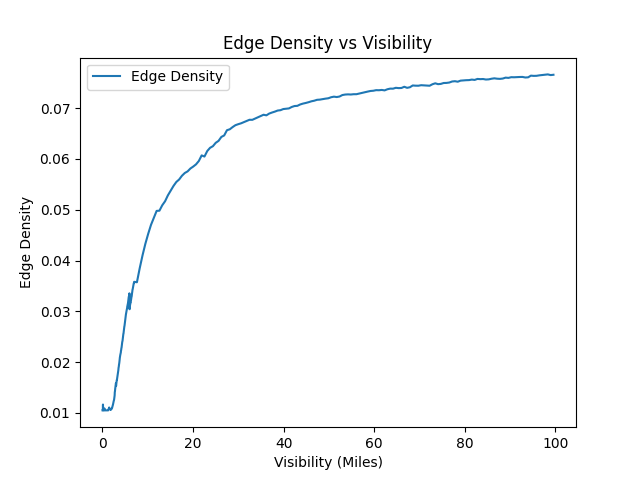
\includegraphics[width=\textwidth]{imgs/edge_density_vs_visibility.png}
    
    \end{subfigure}
    % Mean of Dark Channel Prior vs Visibility
    \begin{subfigure}[b]{0.4\textwidth}
        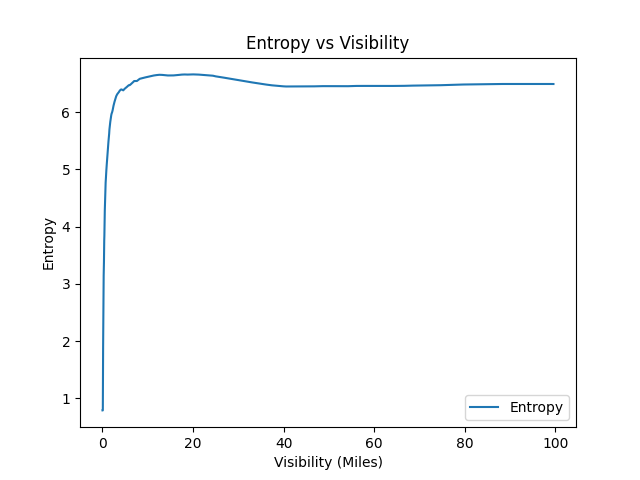
\includegraphics[width=\textwidth]{imgs/entropy_vs_visibility.png}
    \end{subfigure}
    % Mean of Edge Density vs Visibility
    \begin{subfigure}[b]{0.4\textwidth}
    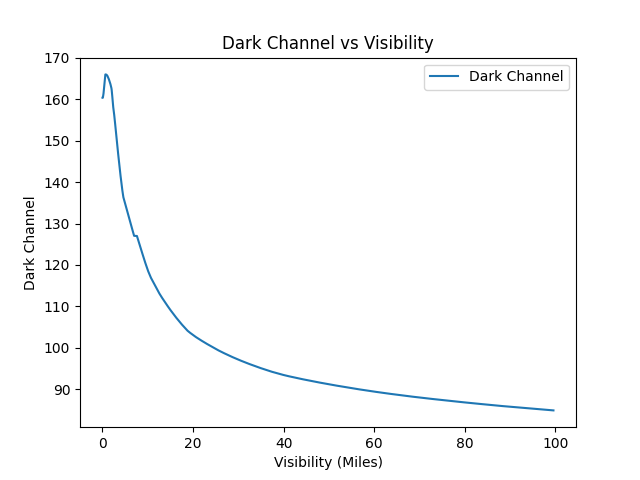
\includegraphics[width=\textwidth]{imgs/dark_channel_vs_visibility.png}
        
    \end{subfigure}
    % Mean of FFT Magnitude vs Visibility
    \begin{subfigure}[b]{0.4\textwidth}
        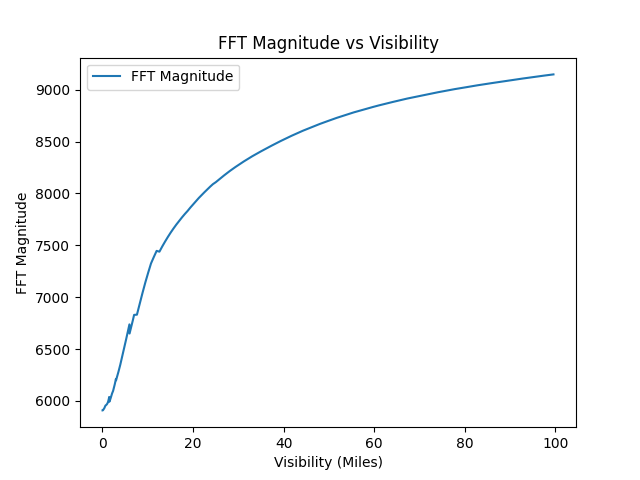
\includegraphics[width=\textwidth]{imgs/fft_magnitude_vs_visibility.png}
    \end{subfigure}
    \caption{Impact of Visibility Degradation on Edge Density (a), Entropy map (b), Dark Channel Prior (c), and FFT Magnitude (d) vs Visibility in Miles}
    \label{fig:mean_of_features}
\end{figure}

 In Figures~\ref{fig:impact_vis_deg_features}, \ref{fig:mean_of_features}, we show the impact of visibility degradation on various modalities of the same scenery. Each row shows one modality, while each column refers to a visibility bin.
\subsection{Fusing Modalities}
Numerous methods have been proposed in the literature for fusing different modalities and multiple stream networks \cite{akkus2023multimodal, radford2021learning, jia2021scaling}. These methods range from simple concatenation of different inputs from the input space to fusion at different levels of the model architecture. 

Early fusion \cite{huang_fusion_2020}, where we concatenate or preprocess all input streams in the input space, then feed it to a single feature extractor which extracts as much information as possible before feeding it to a decoder, classifier head, or projection head. While this method is the simplest method one can use to fuse different modalities, it has many limits where the feature-extracted model might learn to ignore most of the modalities from the early layers and be dominated by only one modality.

Another approach, widely used in the literature, involves feeding the different modalities into separate encoder layers before fusing all the extracted embeddings \cite{huang_fusion_2020}. In this approach, the model learns to extract useful features from each modality before they are fused, thus preventing one modality from dominating the feature space. But one of the biggest benefits of using this type of architecture is the ability to use recent advancements in representation learning, where each modality is processed through its own encoder, then using either contrastive learning to pre-train all the encoders to align together, or using the unsupervised representation learning where fusion happens in the between the encoder and decoder layer or right from the get-go.

Late fusion is another type of fusion \cite{huang_fusion_2020}, where each modality is passed through its own encoder, decoder, or any number of layers until the decision layer (e.g., binary classification). Fusion is then performed either by voting between different models or by taking the mean of the different decisions.

\subsubsection{Multimodal Fusion Methods}
In the literature, various techniques such as Tensor Fusion \cite{zadeh2017tensorfusionnetworkmultimodal}, Low-Rank Fusion \cite{liu2018efficientlowrankmultimodalfusion}, and attention \cite{NEURIPS2021_76ba9f56} have been proposed \. Although each method has its own advantages and disadvantages, self-attention has emerged as the cornerstone for many recent large-scale methods. While it requires more training data, its computation is significantly low compared to methods like tensor fusion.


\subsubsection{SeeNN Multimodal Fusion Framework}

\label{subsub:proposed}


\begin{figure}
    \centering
    \begin{subfigure}[b]{0.64\textwidth}
        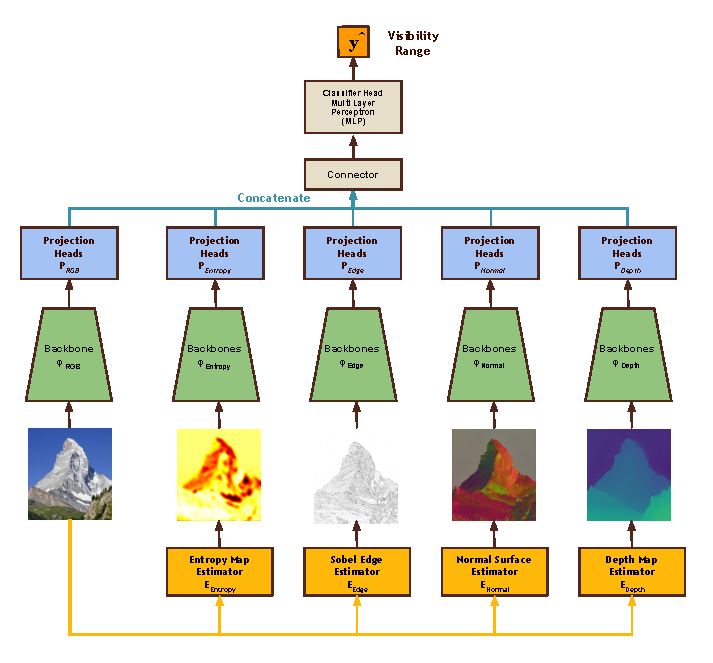
\includegraphics[width=\textwidth]{imgs/SeeNN_Expanded.pdf}
    \caption{}
    \end{subfigure}
    \begin{subfigure}[b]{0.2\textwidth}
        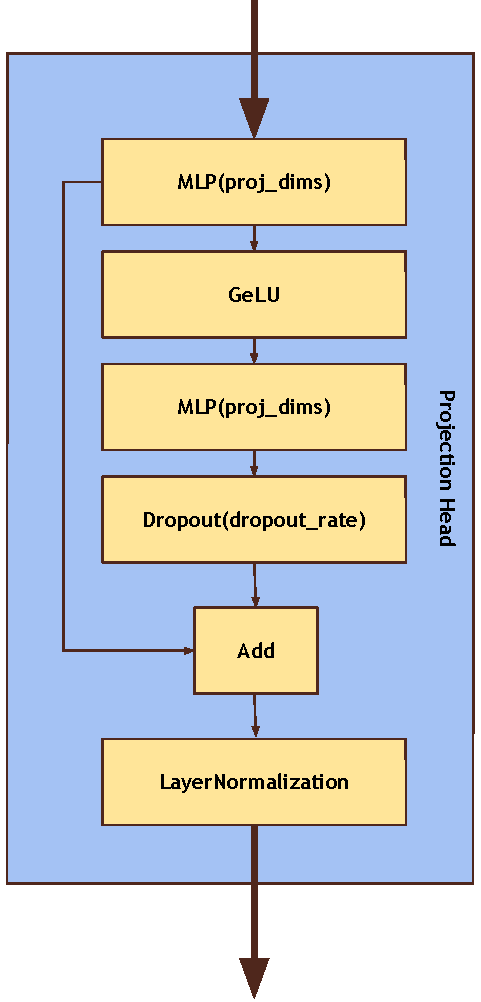
\includegraphics[width=\textwidth]{imgs/Projection Head.pdf}
    \label{fig:projection_head}
        \caption{}
    \end{subfigure}
\caption{
(a) SeeNN Framework: The framework first extracts features (entropy map, surface normals map, edge map, depth map) from the input image. Separate encoders $\phi_{m}(\cdot)$ ($\phi_{m}(\cdot)$ denotes modality encoders) process these features followed by a projection head (b), followed by fusion of these features through a Connector and prediction via a classifier $\mathbf{\hat{y}}$.
(b) Projection Head: The input vector is transformed by an MLP (Multi-Layer Perceptron) with a non-linear activation function (GeLU) and dropout for regularization.
}
\label{fig:seeeNN}
\end{figure}

The proposed SeeNN framework (Figure~\ref{fig:seeeNN}) integrates multimodal DL techniques to process the images alongside the multiple modalities. 
First, each input RGB image \( I \) undergoes a series of transformations through modality estimators to produce a depth map \( E_d(I) \), a normal surface map \( E_n(I) \), an edge detection map \( E_e(I) \), and an entropy map \( E_s(I) \). Each of these modalities captures distinct characteristics of the input, providing diverse perspectives on the image's content.

Let $m$ denote one of the modalities (generated depth map $depth$, normal surface $normal$, entropy map $entropy$, edge map $edge$, and RGB image $rgb$). We implement different backbone models $\Phi_{m}(\cdot)$ for each modality input $X_m$. 
We use DenseNet121 \cite{huang_densely_2018} as the architecture for all $\Phi_{m}$ and we feed the resulted embedding from each encoder to a projection head $P_m$ which consists of an MLP with a non-linear
activation function (GeLU) and dropout for regularization, followed by a layer normalization which is a crucial step to align the feature representations, mitigating the risk of dominance by any single modality due to varying magnitudes of feature values, then we obtain a feature vector \( F_m \).

We apply this process to RGB image $X_{rgb}$, depth \( X_{depth} \), normal surface  \( X_{normal} \), entropy  \( X_{entropy} \), and edge map \( X_{edge} \) to obtain $F_{rgb}$, $F_{depth}$, $F_{normal}$, $F_{entropy}$, $F_{edge}$, respectively. 

Following projection heads, the SeeNN framework concatenates these embeddings into a single, comprehensive feature vector \( F \). 
The concatenation is represented as \( F = [F_{rgb}, F_{depth}; F_{normal}; F_{entropy}; F_{edge}] \), which is then fed to the connector $C$ that is responsible for fusing these modalities.
We then apply an MLP classifier head to get the final prediction $\hat{y}$.  

When it comes to the connector, we primarily used two methods. The first method involves passing the flattened $F$ directly to the MLP, which involves a simple fusion of the different features. The second method utilizes an attention block to perform self-attention on $F$, followed by flattening the output and feeding it to the MLP head.


\subsubsection{Experimental Setup}
For our study, we use our collected dataset, SeeSet v1 \ref{sec:seeset}, made of 320 distinct views collected across 20 locations with different land covers, each with visibility ranging from 0 to 100 miles. We split the dataset into two subsets using the holdout approach, where we select all the views from specific locations, and hid them from the model during validation, to ensure that our model doesn't overfit the sceneries and vegetation and learn to estimate the visibility based on the degradation of the image \cite{Bouhsine2022}. This resulted in $100,350$ instances for training and $15,750$ for validation. Each image in the dataset is preprocessed to an input shape of $224 \times 224$ pixels.

We leverage the Omnidata models to preprocess RGB images and export the estimated Depth Map and the Normal Surface \cite{eftekhar2021omnidata}, which is based on the DPT-Hybrid architecture \cite{ranftl2021vision} and is similar to the approach taken in the literature to generate pseudo labels from RGB to pre-train multimodal models \cite{bachmann2022multimae, wang2024largescale}. 
For the other modalities, i.e., edge map and entropy map, the RGB images are initially processed through the hand-made estimators (Figure~\ref{fig:seeeNN}).

We train all models for 100 epochs and we use the Adam optimizer with a learning rate of $0.001$. For all models, we set the batch size to $32$.
